\section{Nonlinear systems}

In cases where the system exhibits nonlinearity, we can still apply a similar approach, but now necessitating a nonlinear software sensor.
\begin{figure}[H]
    \centering
    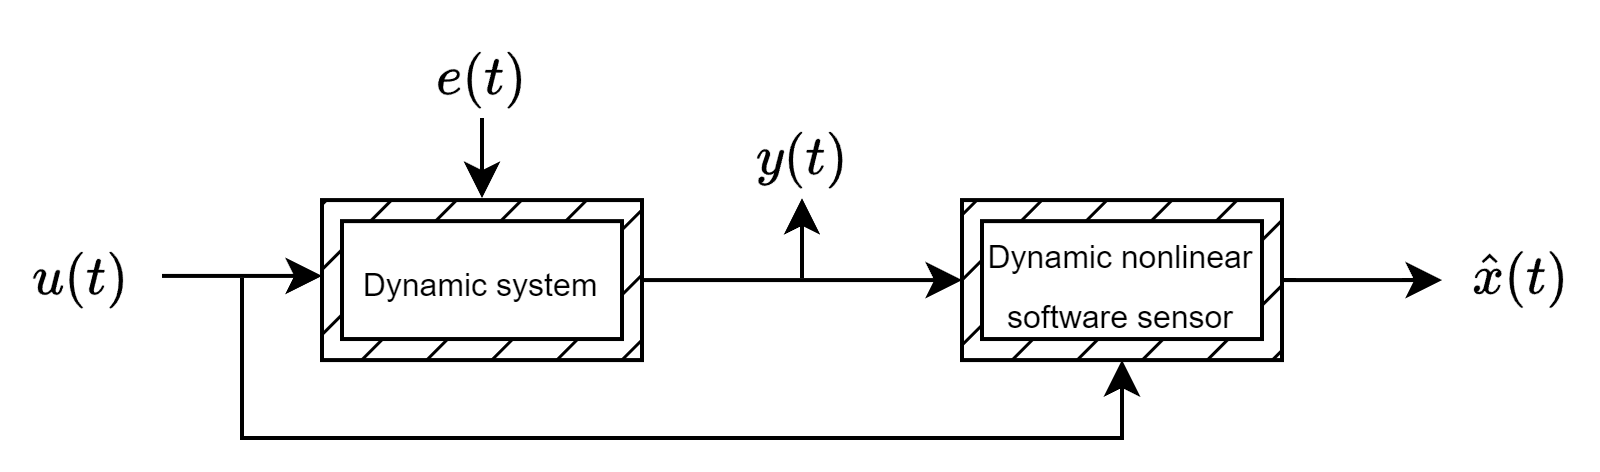
\includegraphics[width=0.75\linewidth]{images/lin.png}
    \caption{Nonlinear software sensor}
\end{figure}
\noindent There exist four potential architectures commonly employed to address nonlinear problems.

\subsection{Neural Network architecture}
In this framework, a dynamical Neural Network is employed:
\begin{figure}[H]
    \centering
    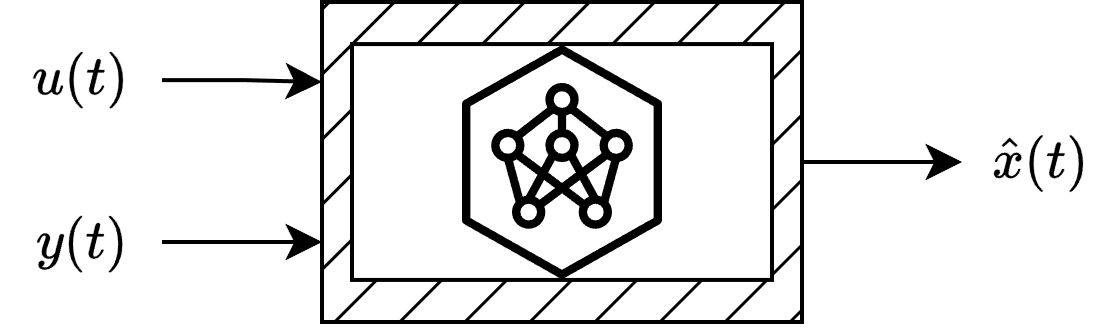
\includegraphics[width=0.4\linewidth]{images/nn.png}
    \caption{Neural Network}
\end{figure}
\noindent Each neuron within the network can be either static or dynamic:
\begin{figure}[H]
    \centering
    \begin{subfigure}{0.49\textwidth}
        \centering
        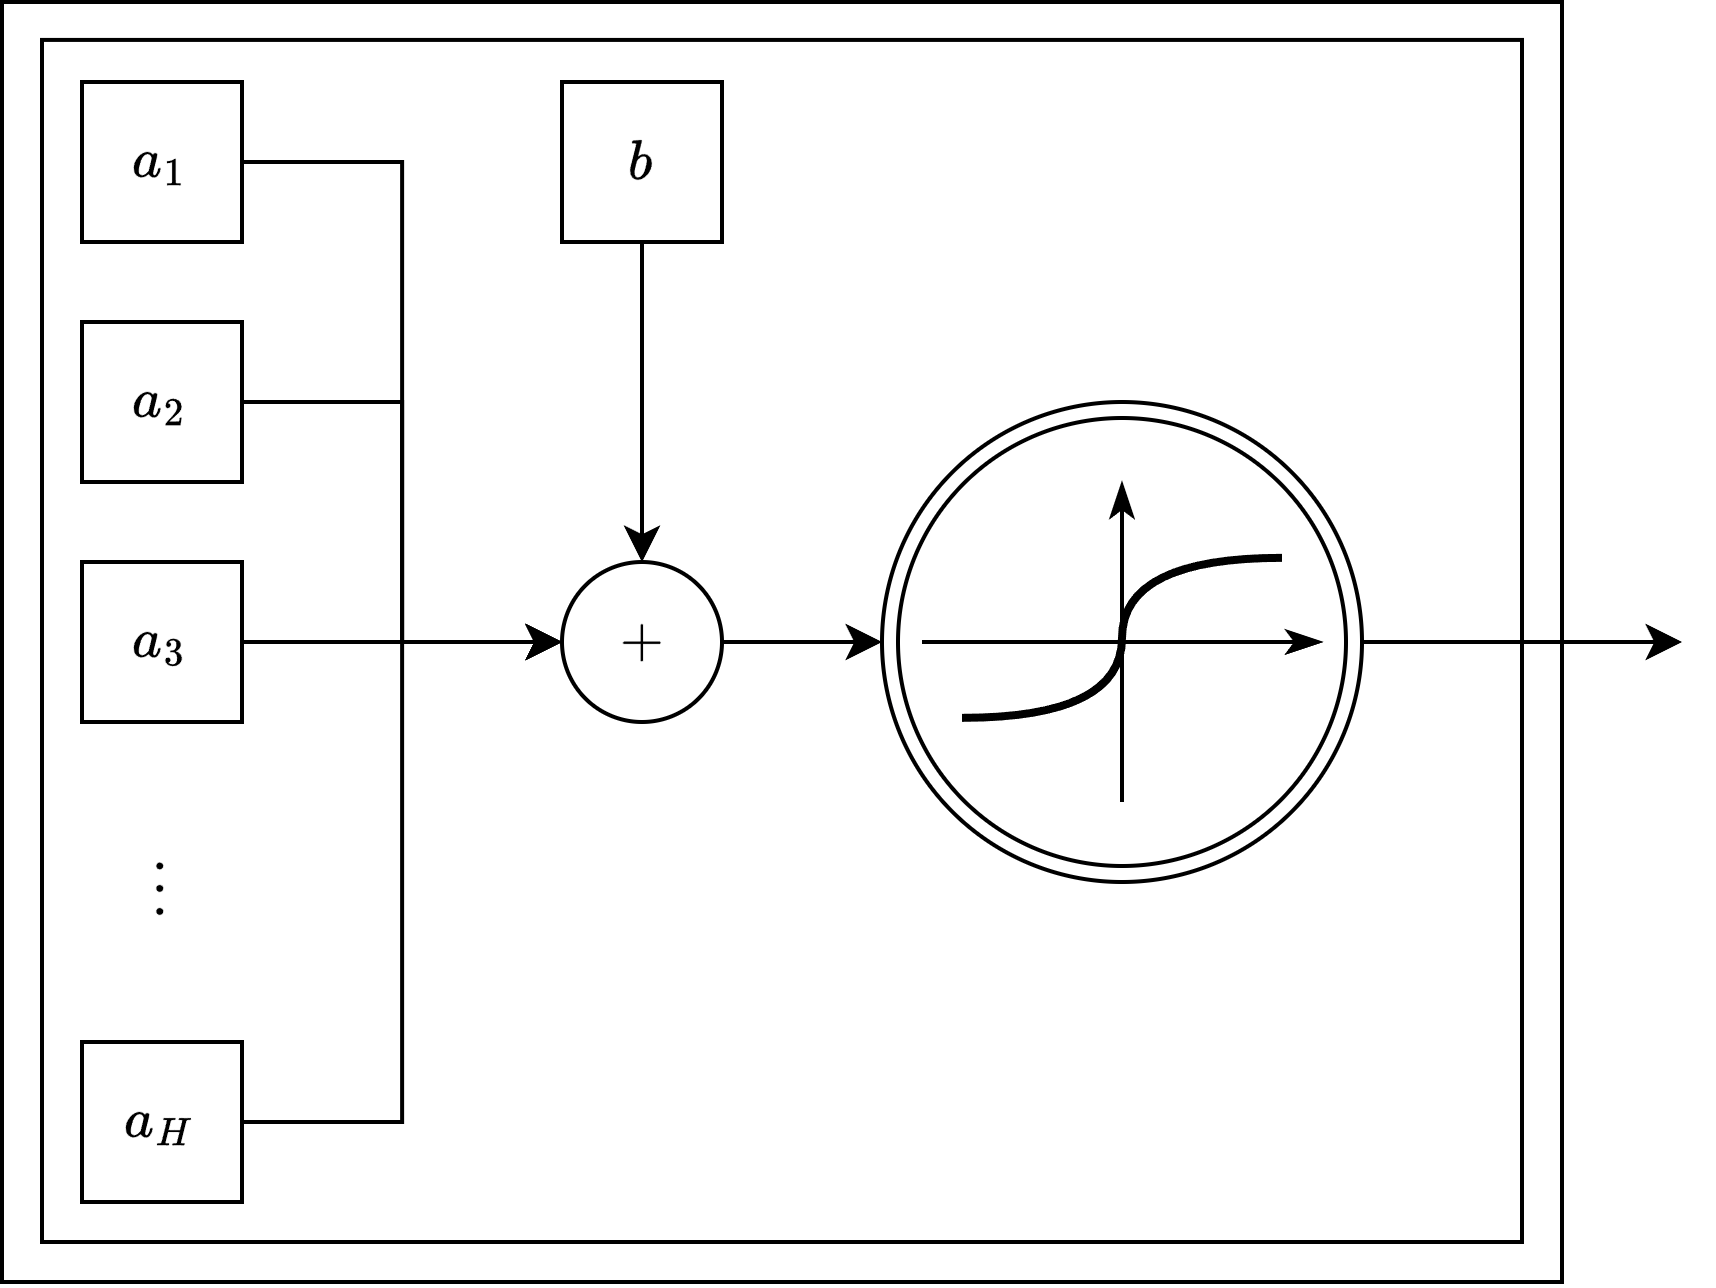
\includegraphics[width=0.75\linewidth]{images/snn.png} 
        \caption{Static Neuron}
    \end{subfigure}
    \begin{subfigure}{0.49\textwidth}
        \centering
        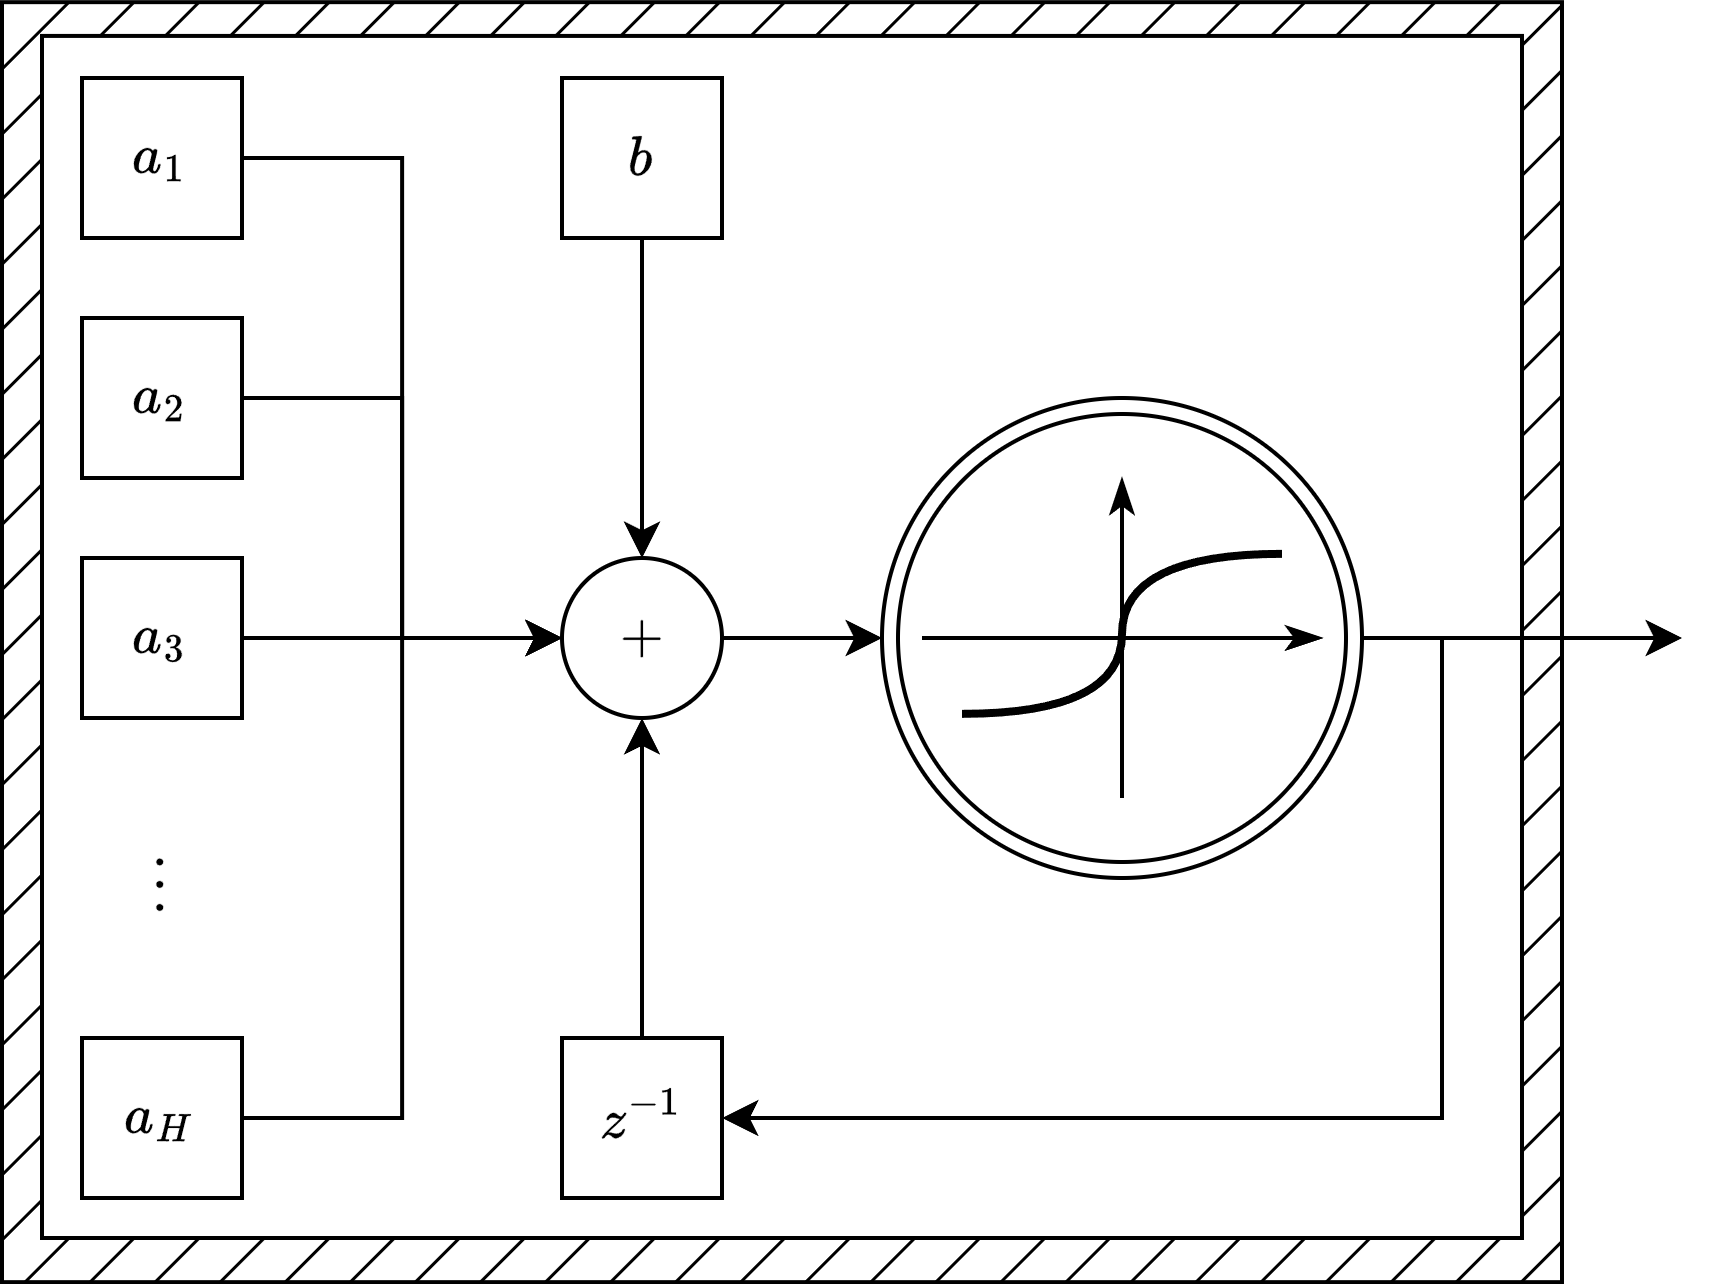
\includegraphics[width=0.75\linewidth]{images/dnn.png}
        \caption{Dynamic Neuron}
    \end{subfigure}
    \caption{Neurons}
\end{figure}

\noindent This architecture is intuitive and versatile, but not widely used in practice due to:
\begin{itemize}
    \item High computational demand for training and optimization.
    \item Lack of guarantee regarding convergence and stability of the resulting Neural Network.
\end{itemize}

\subsection{Finite Impulse Response filter architecture}
The software sensor is divided into a static nonlinear part and a dynamic nonlinear part utilizing a non-recursive Finite Impulse Response Filter-like scheme:
\begin{figure}[H]
    \centering
    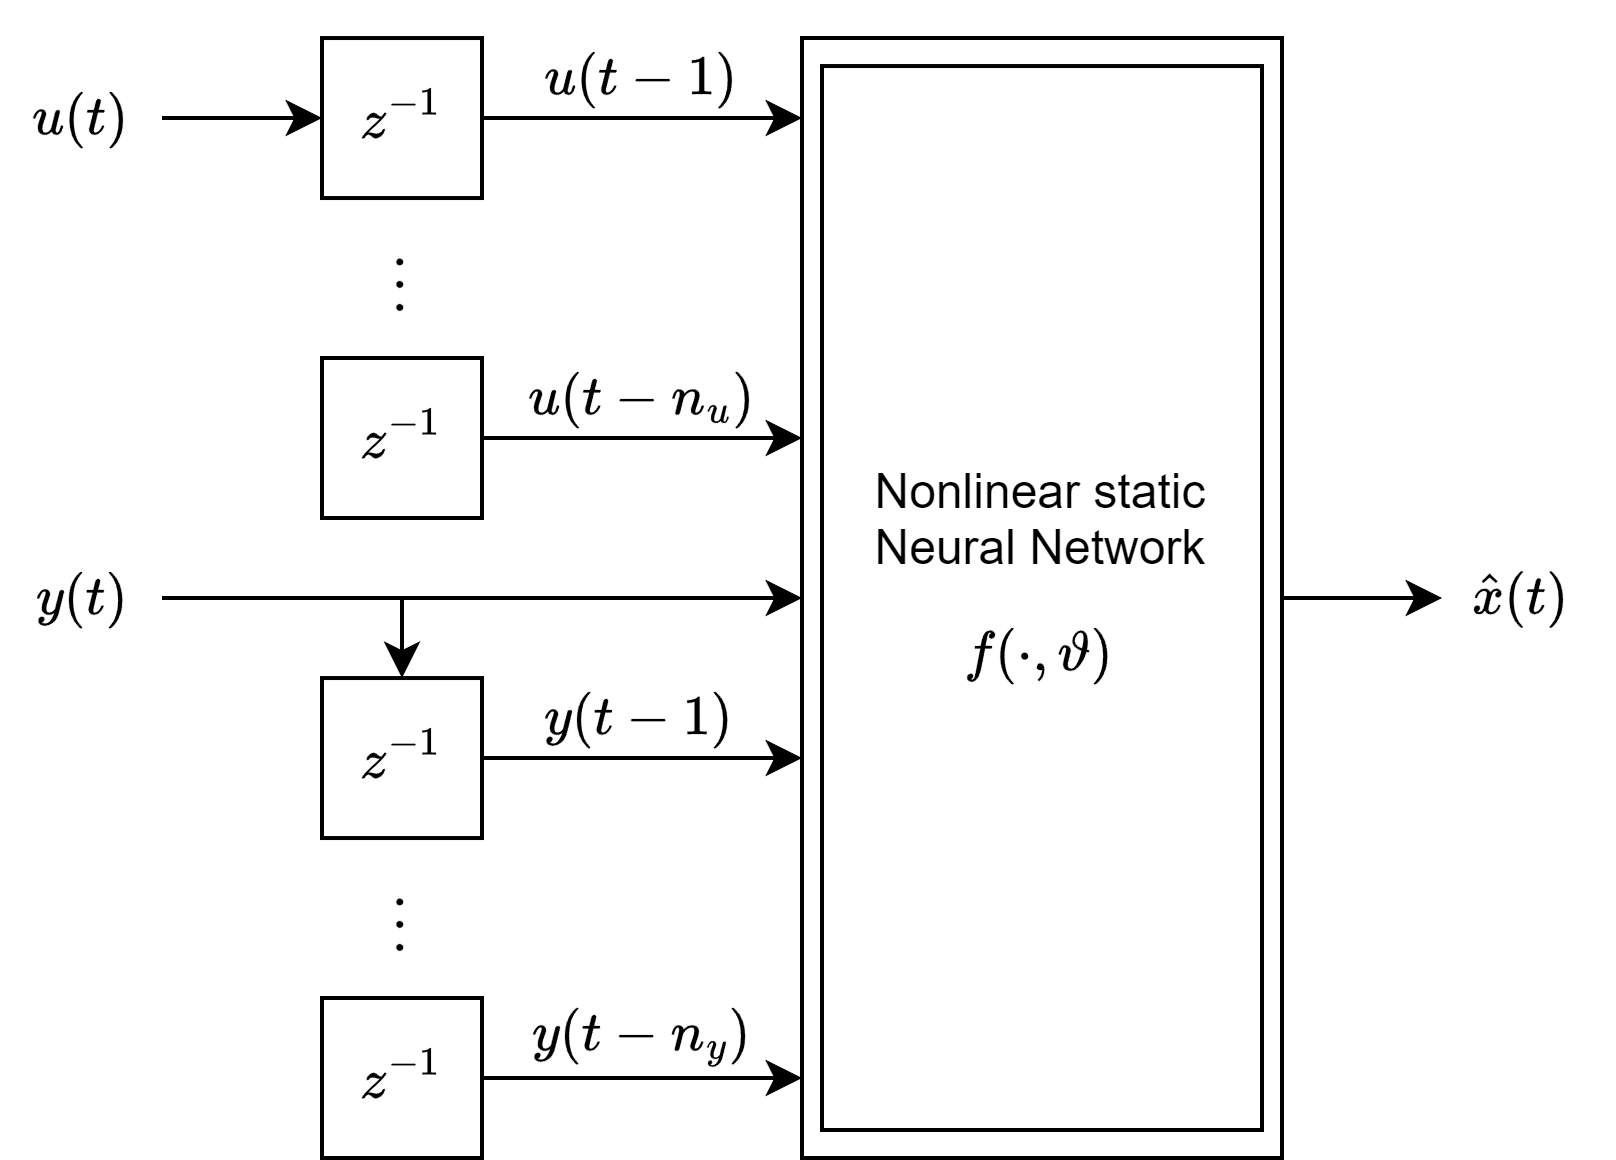
\includegraphics[width=0.5\linewidth]{images/split.png}
    \caption{Input and output splitting}
\end{figure}

\noindent The inputs and outputs are treated as linear dynamic systems, while the block represents a nonlinear static parametric system. 
Consequently, training is solely focused on the static nonlinear Neural Network component.

The training process is limited to the static nonlinear Neural Network, ensuring stability by design.

It's important to note that in the case of multiple input multiple output systems, where:
\[u(t)=\begin{bmatrix} u_1(t) \\ u_2(t) \\ \vdots \\ u_m(t) \end{bmatrix} \quad y(t)=\begin{bmatrix} y_1(t) \\ y_2(t) \\ \vdots \\ y_p(t) \end{bmatrix} \quad x(t)=\begin{bmatrix} x_1(t) \\ x_2(t) \\ \vdots \\ x_n(t) \end{bmatrix}\]
As a result, the input-output size can be significant.

\subsection{Infinite Impulse Response filter architecture}
To address the challenge of large mapping input-output sizes, we can adopt the previous architecture but incorporate recursion, resembling an Infinite Impulse Response filter scheme:
\begin{figure}[H]
    \centering
    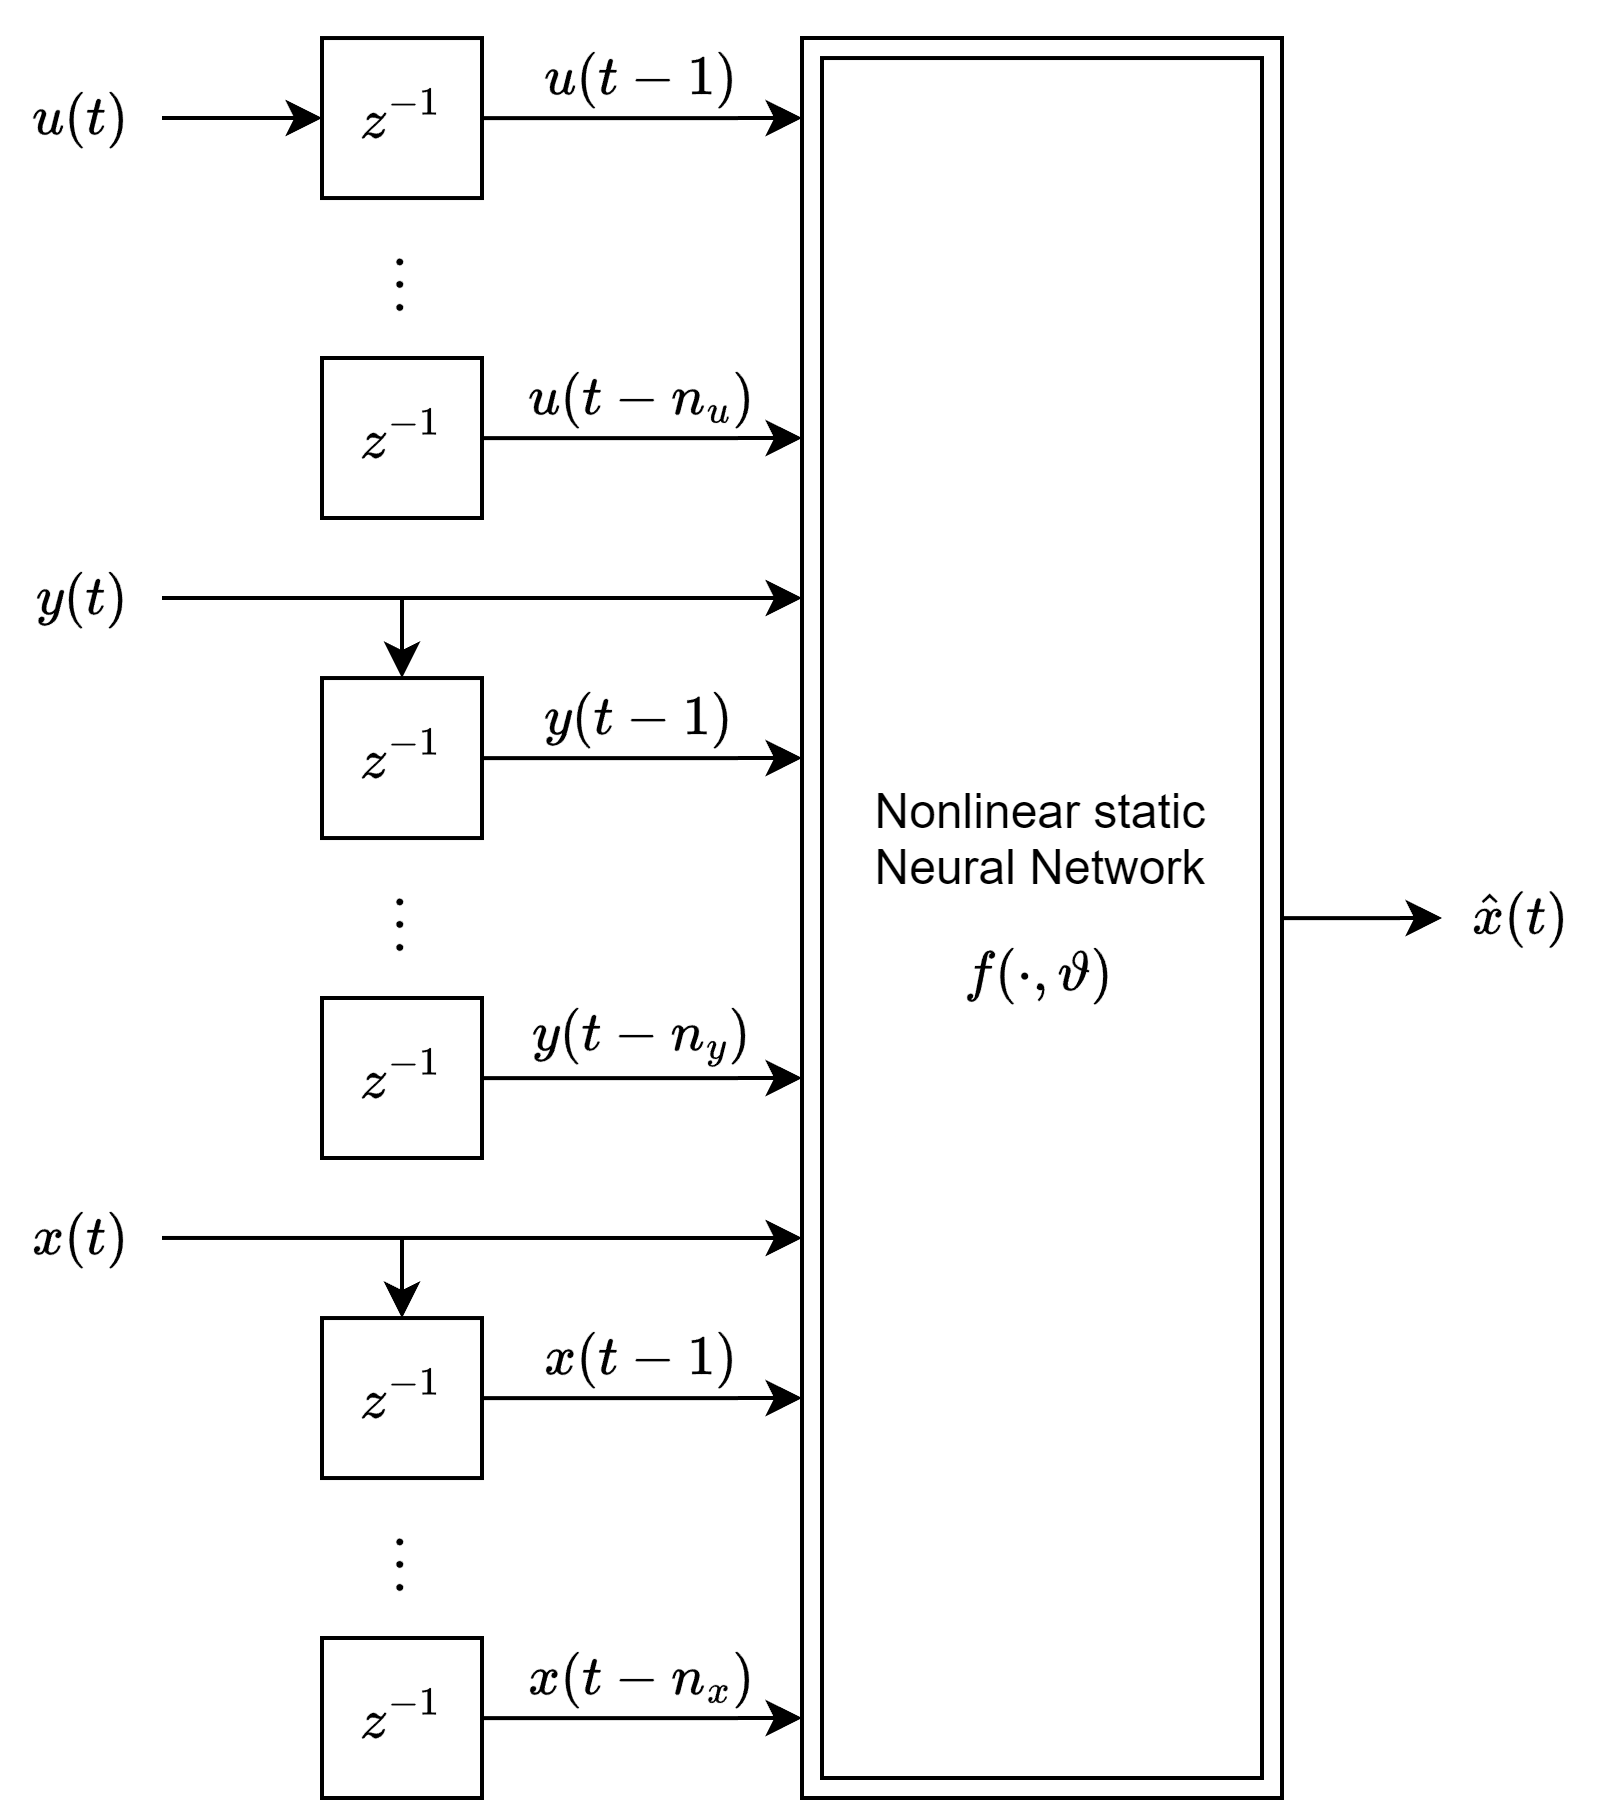
\includegraphics[width=0.4\linewidth]{images/split1.png}
    \caption{Training input and output splitting with recursion}
\end{figure}
\noindent This architecture features a recursive state component that considers past output values.
The advantage lies in the potential reduction of $n_u$ and $n_y$ dimensions.
However, a notable disadvantage arises during production, as $\mathbf{x}(t)$ is no longer available after training. 
Consequently, it must be substituted with feedback on $\hat{\mathbf{x}}(t)$:
\begin{figure}[H]
    \centering
    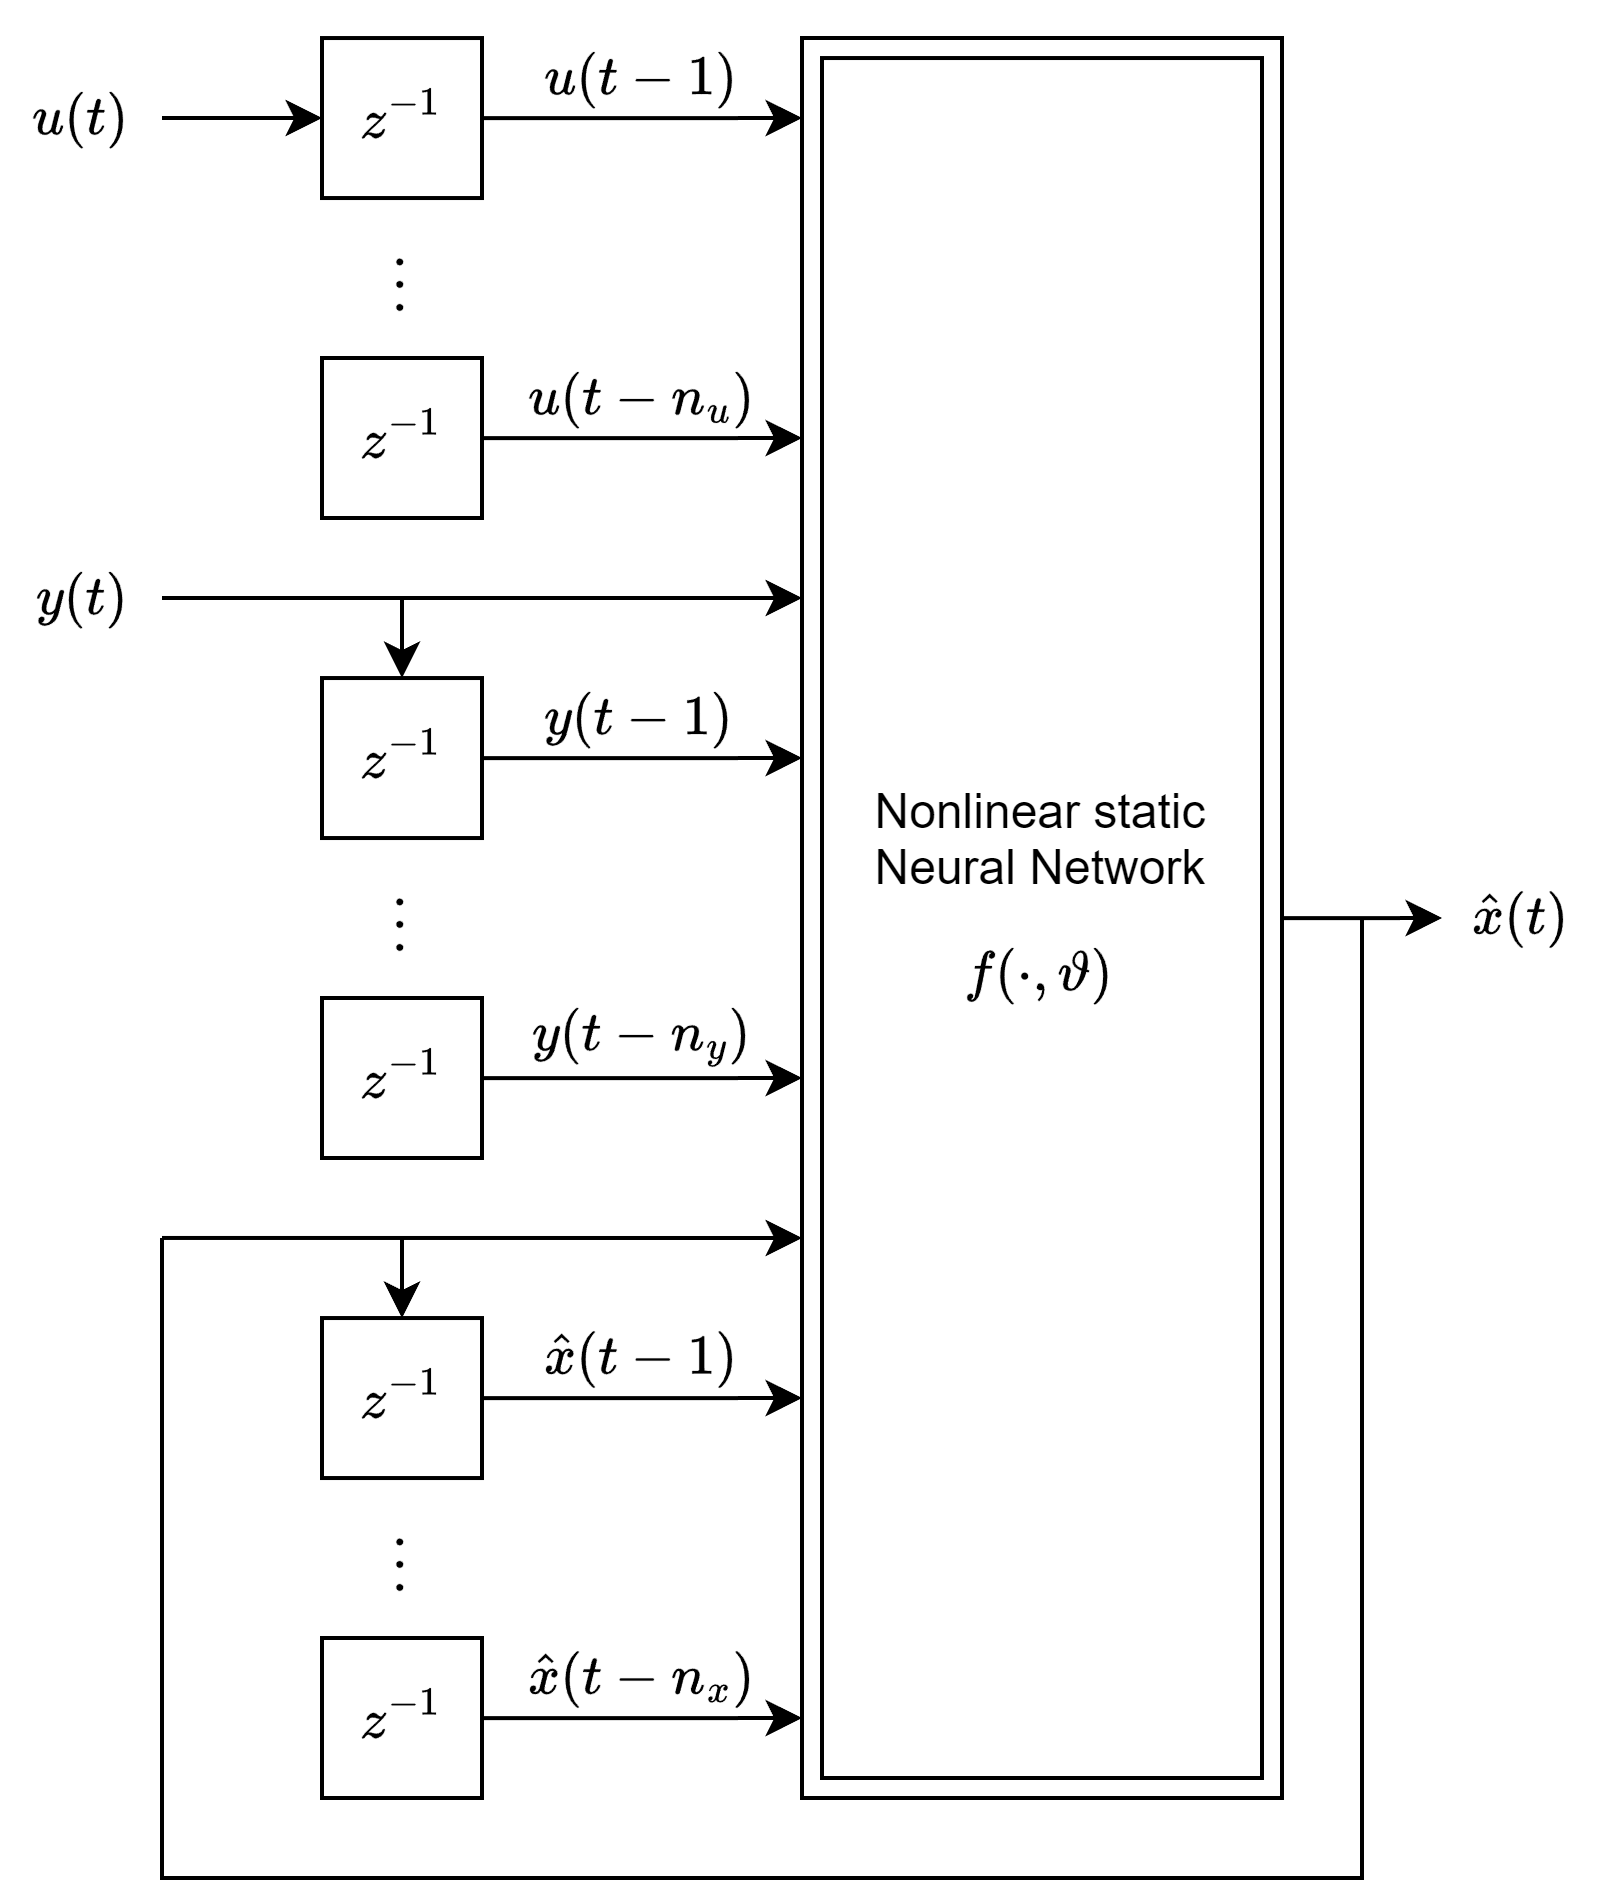
\includegraphics[width=0.4\linewidth]{images/split2.png}
    \caption{Production input and output splitting with recursion}
\end{figure}
\noindent This feedback mechanism on $\hat{\mathbf{x}}(t)$  introduces the potential for system instability.

\subsection{Meta architecture}
This architecture represents a modification incorporating prior knowledge of the system gleaned from the previous three architectures.
The concept involves splitting the system into two distinct parts:
\begin{figure}[H]
    \centering
    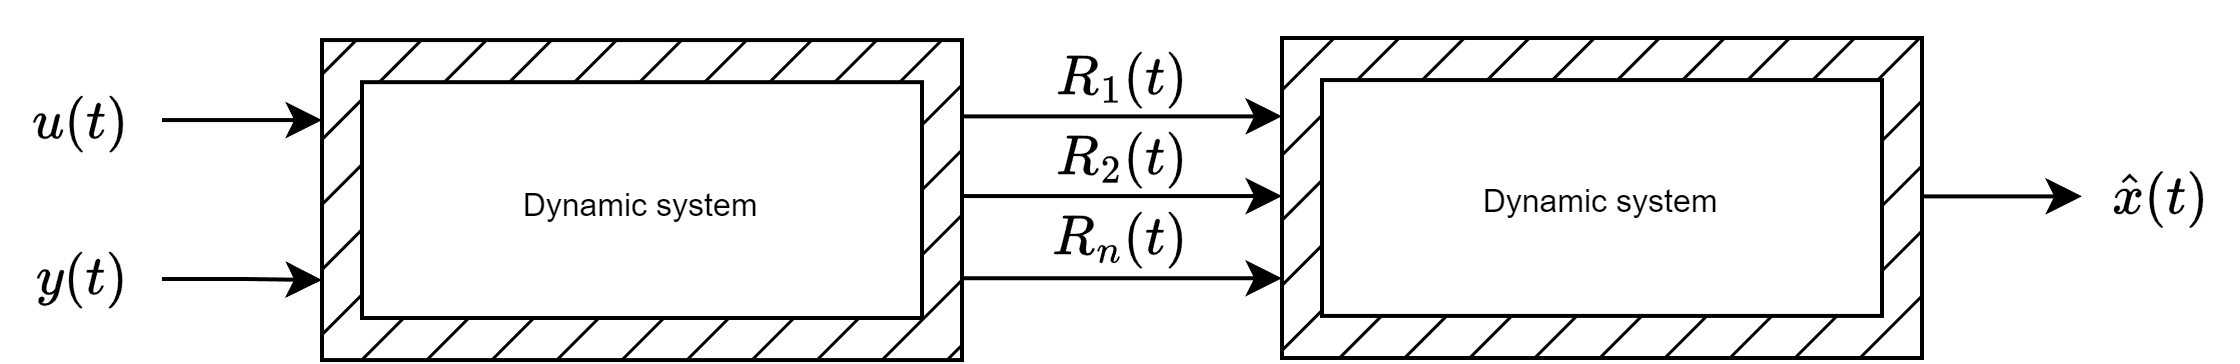
\includegraphics[width=0.75\linewidth]{images/reg.png}
    \caption{Split architecture}
\end{figure}
\noindent The first block serves as a preprocessing stage, wherein $u(t)$ and $y(t)$ are utilized to construct a set of new signals known as regressors $\mathbf{R}(t)$. 

The preprocessing block is built using a priori knowledge, so it is not built using system identification but with know-how on $u(t)$ and $y(t)$. 
The preprocessing block is constructed using a priori knowledge, obviating the need for system identification. 
Typically, the regressors $\mathbf{R}(t)$ are considerably fewer than $u(t)$ and $y(t)$, leading to a substantial reduction in the size of the second block.

If the regressors are judiciously chosen, the second block may remain static. 
This approach offers the advantage of greatly simplifying the estimation process of the second block.